\section{Formální definice kryptografického systému, symetrické a asymetrické šifry. Výpočetně těžké matematické problémy pro~asymetrické šifry.}

\subsection{Definice}

\uline{Kryptografický systém} pro~šifrování zpráv je pětice $(\mathcal{M}, \mathcal{C}, \mathcal{K}, \mathcal{E}, \mathcal{D})$, kde
$\mathcal{M}$ je prostor otevřených zpráv,
$\mathcal{C}$ prostor šifrových zpráv,
$\mathcal{K}$ prostor klíčů,
$\mathcal{E}, \mathcal{D}$ dvojice zobrazení, které každému klíči $k \in \mathcal{K}$ přiřazují transformaci pro~zašifrování zpráv $E$ a~transformaci pro~dešifrování zpráv $D$, kde platí $D(k,E(k,m))=m \ \forall \ k \in \mathcal{K}, m \in \mathcal{M}$.

\uline{Symetrická šifra} je taková šifra, kde pro~každé $k \in \mathcal{K}$ lze z~transformace zašifrování $E_k$ určit transformaci dešifrování $D_k$ a naopak.

\uline{Asymetrická šifra} je taková šifra, kde pro~skoro všechna $k \in \mathcal{K}$ nelze z~transformace pro~zašifrování $E_k$ určit transformaci dešifrování $D_k$.
Bývá zde přítomen tajný klíč $k$, ze~kterého se vhodnou transformací $G$ vygeneruje dvojice parametrů $(e, d)$, která tvoří veřejné a~privátní klíče ($k_\text{pub}$, $k_\text{priv}$).
Ty parametrizují transformace šifrování a dešifrování.

\subsection{Matematické problémy asymetrických šifer}

\subsubsection{Problém diskrétního logaritmu}

Rovnice $c \equiv g^m \mod p$ je výpočetně jednoduchá a rychlá, získání $m$ z~$c$ je naopak složité.

DLP využívají protokoly Diffie-Hellman, ElGamal, DSA, ECDL, ECDSA, \dots

Mezi algoritmy řešení patří brute-force, baby step--giant step, Pollardův $\rho$ algoritmus, funkční síto, \dots

\subsubsection{Problém faktorizace}

Faktorizace je proces převodu složeného čísla na~jeho prvočíselné složky.

FP využívá například RSA.

Mezi algoritmy řešení patří brute-force, Pollardůvo $\rho$ algoritmus, Pollardův $\rho - 1$ algoritmus, Lehmannova metoda, kvadratické síto, \dots


\clearpage
\section{Služby bezpečnosti zajišťované kryptografickými prostředky, kryptografické mechanismy, které tyto služby zajišťují.}

\subsection{Služby}

\uline{Zabezpečení důvěrnosti dat} (\emph{data confidentiality}) je ochrana obsahu proti analýze.
Může jít o~zajištění důvěrnosti přenosu zpráv, spojení, toku dat nebo služby selektivní důvěrnosti (které chrání pouze část informace).
\uline{Zabezpečení integrity dat} (\emph{data integrity}) je ochrana proti neautorizované modifikaci.
Slabá integrita: modifikace zprávy šumem, změna pořadí paketů, náhodná duplicita (kontrolní součet, CRC, pořadové číslo).
Silná integrita: podvržení zprávy, úmyslné pozměnění zprávy; bez~oprav a s~opravami.

\uline{Autentizace} (\emph{authentication}) je proces ověření identity entity.
\emph{Peer Entity Authentication} ověřuje uživatele,
\emph{Data Origin Authentication} ověřuje všechna data a eliminuje např. útoky opakováním.

\uline{Řízení přístupu} (\emph{access control}) je možnost povolit či odepřít použití určitého zdroje určitému subjektu.

\uline{Ochrana proti odmítnutí původu zprávy} (\emph{non-repudiation}) zajišťuje důkaz o~původu dat a dokazuje původ nebo doručení.

\subsection{Mechanismy}

Šifrování, digitální podpisy, řízení přístupu, mechanismy integrity dat, výměna autentizační informace, padding, řízení směrování, ověření třetí stranou.

\begin{table}[ht]
	\centering
	\onehalfspacing

	\begin{tabular}{|l|cccccccc|}
		&
		\begin{sideways}šifrování\end{sideways} &
		\begin{sideways}podpis\end{sideways} &
		\begin{sideways}řízení přístupu\end{sideways} &
		\begin{sideways}integrita\end{sideways} &
		\begin{sideways}autentizace\end{sideways} &
		\begin{sideways}padding\end{sideways} &
		\begin{sideways}řízení směrování\end{sideways} &
		\begin{sideways}ověření třetí stranou\end{sideways} \\
		\hline\hline
		%                              š   p   ř   i   a   p   ř   o
		autentizace spojení          & X & X &   &   & X &   &   &   \\
		autentizace odesílatele      & X & X &   &   &   &   &   &   \\
		řízení přístupu              &   &   & X &   &   &   &   &   \\
		důvěrnost spojení            & X &   &   &   &   &   &   &   \\
		důvěrnost přenosu zpráv      & X &   &   &   &   &   & X &   \\
		selektivní důvěrnost         & X &   &   &   &   &   & X &   \\
		důvěrnost toku dat           & X &   &   &   &   & X & X &   \\
		integrita spojení s~opravou  & X &   &   & X &   &   &   &   \\
		integrita spojení bez~opravy & X &   &   & X &   &   &   &   \\
		selektivní integrita spojení & X & X &   & X &   &   &   &   \\
		integrita přenosu zpráv      & X & X &   & X &   &   &   &   \\
		nepopiratelnost odesílatele  & X & X &   & X &   &   &   & X \\
		nepopiratelnost doručení     & X & X &   & X &   &   &   & X \\
	\end{tabular}

	\caption{Matice mechanismů bezpečnosti}
\end{table}


\clearpage
\section{Kryptograficky bezpečné generátory náhodných čísel: požadavky, hodnocení bezpečnosti, příklady realizace.}

\subsection{Požadavky}

\uline{Next-bit test}: je-li známo prvních $k$ bitů náhodné posloupnosti, neexistuje žádný algoritmus s~polynomiální složitostí, který by dokázal předpovědět $(k + 1)$ bit s~pravděpodobností vyšší než 1/2.

\uline{State compromise}: i~když je zjištěn vnitřní stav generátoru (celý nebo z~části), nelze zpětně zrekonstruovat dosavadní vygenerovanou posloupnost.
Navíc, pokud do~generátoru za~běhu vstupuje další entropie, nemělo by být možné ze~znalosti vnitřního stavu předpovědět vnitřní stav v~následujících iteracích.

Vetšina používaných PRNG tyto požadavky splňuje jen za~určitých podmínek.

\subsection{Hodnocení bezpečnosti}

Entropie je veličina popisující míru náhodnosti: jak obtížné je hodnotu (číslo, posloupnost) uhodnout.
Míra nejistoty (nepředvídatelnosti) závisí na~pravděpodobnostech možných výsledků procesu který ji generuje.

Je~dána vztahem
$$H(X) = -\sum_{i-1}^n p_{i} \log_2 p_{i}$$
kde
$X$ je generovaná hodnota,
$p_1, \dots, p_n$ jsou pravděpodobnosti hodnot $X_1, \dots, X_n$ které je daný generátor schopen vygenerovat.

Hodnota entropie vyjadřuje obsažené množství informace v~bitech.
Vztahuje se ke~schopnosti útočníka předpovídat vygenerovanou hodnotu: pokud ji zná s~jistotou, entropie je nulová.
Naopak má generátor entropii maximální tehdy, pokud se pro~danou délku výstupu generují všechny možné posloupnosti, každá se~stejnou pravděpodobností.

\subsubsection{Statistické testy}
Lze jimi prokázat, že generátor \uv{Nejspíše není kvalitní}, odhalují slabiny. Pokud projde testem, neznamená to, že je RNG kvalitní. Tvoří se sady testů, testují hypotézy na určité hladině významnosti.

\begin{itemize}
    \item Frekvenční test -- přibližně stejně jedniček a~nul
    \item \uv{runs} test -- jsou posloupnosti opakujících se 0 a~1 za sebou náhodné? (odpovídají náhodné poslounosti?)
    \item Poker test: rozdělení na \(k\)-tice, vyhodnocuje se četnost jednotlivých sekvencí
    \item Test hodnosti matic -- disjunktní podmatice a~lin.\,závislost jejich vektorů
    \item Spektrální test -- diskrétní Fourierova transformace (periodicita bude odhalena)
    \item Maureův test -- lze posloupnost komprimovat?
    \item \uv{Monkey} test -- generování symbolů abecedy, zjišťuje se četnost předem definovaných \uv{slov} ze symbolů
    \item \dots
\end{itemize}

Sady testů:
\begin{itemize}
    \item Diehard
    \item Dieharder
    \item FIPS 140-1
    \item FIPS 140-2
    \item NIST Statistical Test Suite
\end{itemize}


\subsection{Příklady realizace}

\begin{itemize}
    \item
        Bloková šifra v~režimu čítače: náhodně se zvolí klíč (\emph{seed}) a~počáteční hodnota čítače $i$.
        Zvoleným klíčem se postupně šifrují hodnoty $i$, $i+1$, atd. dokud nedojde k~překročení velikosti bloku (perioda).
    \item
        Hashovací funkce aplikovaná na~čítač: náhodně se zvolí počáteční hodnota čítače $i$.
        Postupně se hashují hodnoty $i$, $i+1$ atd.
        Nesmí dojít k prozrazení počáteční hodnoty čítače.
    \item
        Proudové šifry jsou v~zásadě PRNG, s~jehož výstupem se provádí XOR s~otevřeným textem.
    \item
        Algoritmy založené na~teorii čísel: specializované algoritmy generování u~kterých byl proveden důkaz bezpečnosti.
\end{itemize}


\subsubsection{Pseudonáhodné generátory}

PRNG (\emph{Pseudorandom Number Generators}) jsou definované algoritmicky a~tedy i~deterministicky, a~náhodnost výsledku je tedy pouze zdánlivá.
Mezi jejich výhody patří velká rychlost, lehká realizovatelnost a dobrá nastavitelnost odchylky rozložení; jsou ale málo bezpečné a periodické.


\subsubsection{Kryptograficky bezpečné generátory}

Kryptograficky bezpečné generátory vyžadují pro~generování výstupu skutečně náhodné vstupy (\emph{seed}), na~kterých závisí kvalita výstupu.
V~moderních operačních systémech (Linux) jde např. o~sběr událostí z~pohybu myši a~klávesnice, prodlevy pevných disků a některých přerušení.


\subsubsection{Generátory skutečně náhodných čísel}

TRNG (\emph{True Random Number Generators}) využívají fyzikální nebo hardwarové metody získávání vstupu.
Zdroje entropie jsou klasické nebo kvantové fyzikální jevy.
Mezi jejich výhody patří vysoká bezpečnost a neopakovatelnost; jsou ale pomalé, těžko realizovatelné a ne vždy je možné dostáhnout plně rovnoměrného rozložení.


\clearpage
\section{Hašovací funkce: formální definice, požadované vlastnosti, hodnocení bezpečnosti, příklady algoritmů a použití.}

Hashovací funkce je algoritmus pro~převod vstupních dat do~malého čísla o~předem dané velikosti.
Formálně jde o~funkci $\mathcal{H}(M)$ která převádí libovolně velký vstup $M$ na~řetězec o~délce $n$ bitů.

Používají se v~digitálních podpisech (otisk zprávy), pro~kontrolu integrity a identifikaci (otisk souboru), uložení hesel a klíčů, prokázání autorství, jako způsob rychlého přístupu v~paměti (\emph{hashmap}) nebo jako~pseudonáhodné generátory.


\subsection{Vlastnosti hashovacích funkcí}

Pevná délka výstupu.

Jednocestnost: je jednoduché spočítat $h = \mathcal{H}(M)$, ale velmi složité zjistit $h$ při~znalosti $M$.

Bezkoliznost: je velmi složité nalézt dvě rozdílná $M, M'$ taková že $\mathcal{H}(M) = \mathcal{H}(M')$.
Kolizí prvního řádu (\emph{preimage resistance}) se rozumí nalezení vzoru $M$.
Kolizí druhého řádu (\emph{collision resistance}) se rozumí nalezení dvou vzorů $M, M'$ produkujících stejný hash.


\subsection{Hodnocení bezpečnosti}

K~hodnocení bezpečnosti se užívá matematický model \uv{náhodné orákulum} -- v~závislosti na vstupu vytvoří náhodný výstup, který je ale vždy shodný pro stejný vstup.

Nalezení vzoru má složitost \(O(2^n)\). Nalezení kolize ke dvěma libovolným zprávám má složitost \(O(2^\frac{n}{2})\) -- narozeninový paradox. Nalezení \(r\)-násobné kolize: \(O(2^\frac{n\cdot(r-1)}{r})\). (\(n\) udává délku hašovacího kódu)

Počítač s~velkým výpočetním výkonem může kolize hledat pomocí \uline{útoku hrubou silou}.
Protože jde o~prohledávání obrovského (prakticky nekonečného) prostoru, jde o~pomalý proces.
K~hledání hesel při~znalosti jejich hashů se používají předpřipravené slovníky které vstup řadí dle pravděpodobnosti výskytu.

\uline{Kryptoanalýza} je zaměřená na~vnitřní strukturu hashovací funkce, především na~její kompresní část.
Prolomení bezpečnosti komprese znamená diskreditaci hashovací funkce jako takové a nutnost nahrazení jinou, která bude bezpečnější.


\subsection{Princip iteračních hashovacích funkcí}

Jde o~princip dnes nejčastěji používaný (MD, SHA).

Je založený na~opakovaném použití kompresní funkce $h_i = f(h_{i-1}, M_i)$, kde
$M_i$ je aktuální zpracovávaný blok zprávy $M$,
$h_{i-1}$ je výstup předchozího bloku (případně iniciační vektor\footnote{
    Inicializační vektor není v~tomto případě náhodná hodnota.
    Může se buď spočítat z~hashované zprávy, nebo se použije nějaká konstanta.
});
výstupem je nový částečný \emph{digest}.
Hash vzniká z~konečné hodnoty $h_i$ po~zpracování celé zprávy $M$ (viz obr.~\ref{sha}).


\subsection{Pricip hashovacích funkcí typu houba}

Houba (formálně Keccak) je novější princip používaný rodinou SHA3.

Funguje na~principu nasávání a mačkání (\emph{aborbing and squeezing}).
Při~absorbování se bloky dat XORují s~vnitřním stavem a poté transformují permutační funkcí $f$.
Při~vymačkování se tento stav střídavě čte a~znovu transformuje pomocí $f$ (viz obr.~\ref{keccak}).

Bezpečnost a rychlost je dána parametry $r$ (\emph{rate}) a $c$ (\emph{capacity}): rychlost ovlivňuje velikost částečných vstupů a výstupů, kapacita je neměnná a je modifikována pouze permutací, ne XORováním.

\begin{figure}
    \centering
    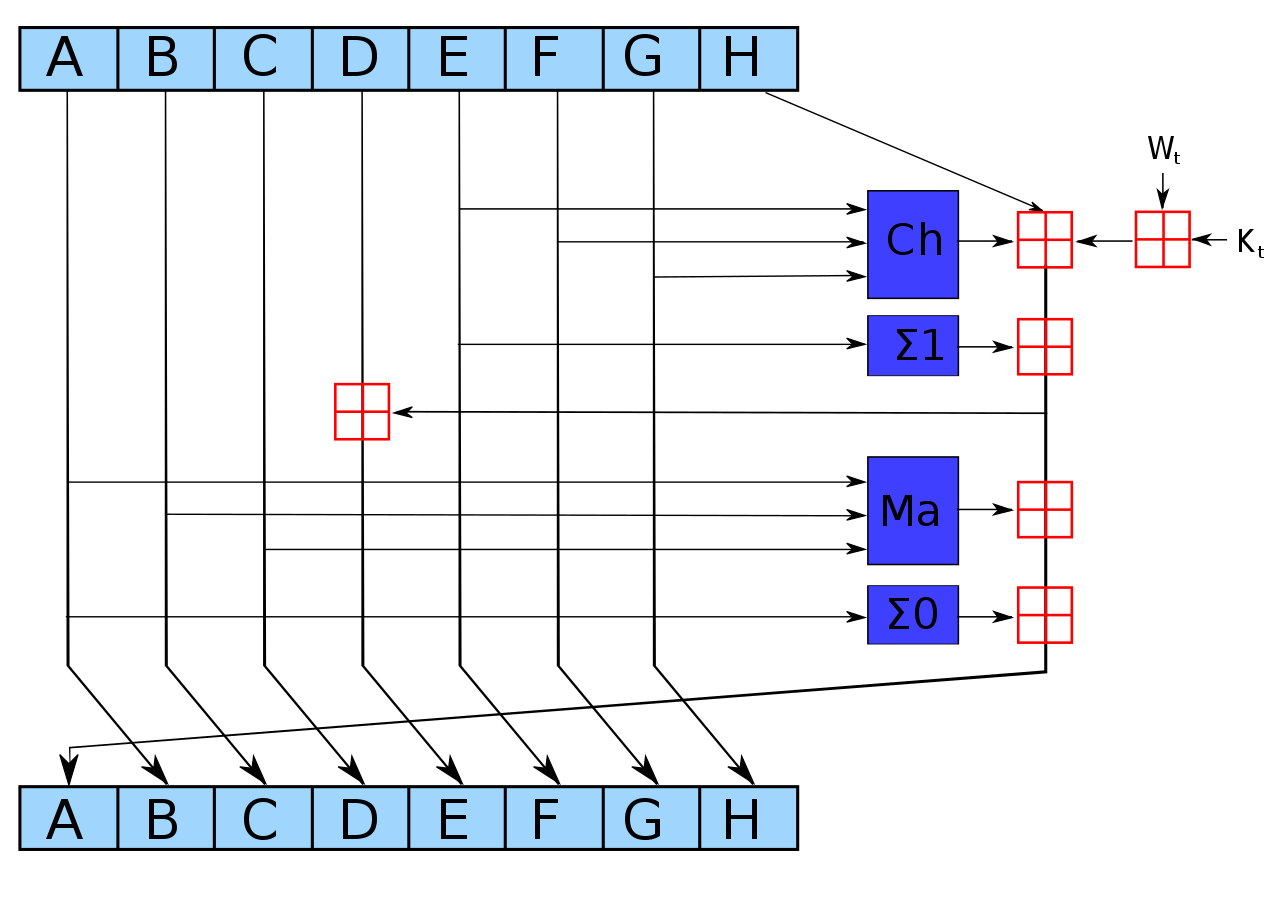
\includegraphics[width=0.6\textwidth]{img/sha-construction}
    \caption{
        Princip zpracování bloku (jedné iterace) v~algoritmu SHA-2.
        Značka $\boxplus$ je sčítání $\mod 2^{32}$ (SHA-256) nebo $\mod 2^{64}$ (SHA-512).
        Modré komponenty reprezentují:
        \\
        $\mathrm{Ch}(E,F,G) = (E \wedge F) \oplus (\neg E \wedge G)$, \\
        $\mathrm{Ma}(A,B,C) = (A \wedge B) \oplus (A \wedge C) \oplus (B \wedge C)$, \\
        $\mathrm{\Sigma_0}(A) = (A \ggg 2) \oplus (A \ggg 13) \oplus (A \ggg 22)$, \\
        $\mathrm{\Sigma_1}(E) = (E \ggg 6) \oplus (E \ggg 11) \oplus (E \ggg 25)$.
        }
    \label{sha}
\end{figure}

\begin{figure}
    \centering
    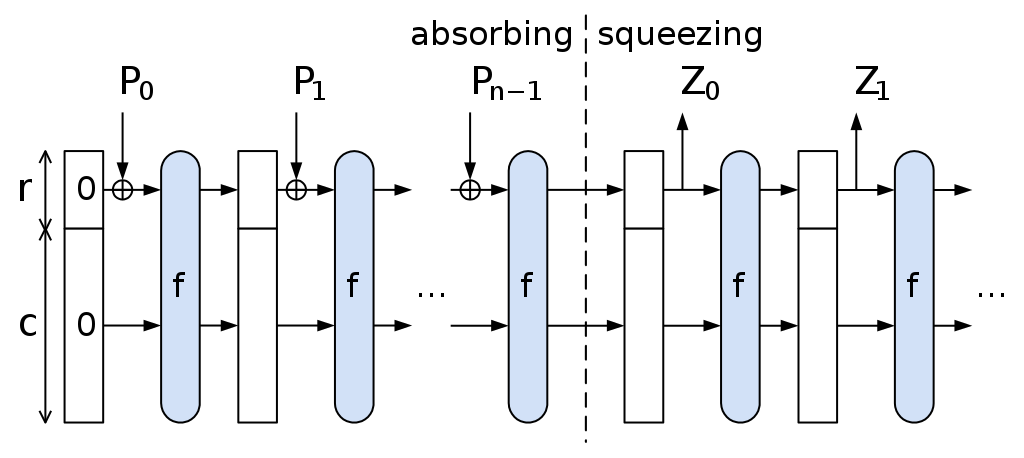
\includegraphics[width=0.6\textwidth]{img/sponge-construction}
    \caption{Princip nasávání a vymačkávání dat algoritmu Keccak.}
    \label{keccak}
\end{figure}


\clearpage
\section{Kryptografie nad eliptickými křivkami, principy, důvody použití, příklady algoritmů.}

Eliptická křivka je množina bodů, která vyhovuje rovnici eliptické funkce.

\subsection{Principy:}
Eliptická křivka (EC) nad množinou reálných čísel je definována jako množina bodů $(x,y)$ vyhovujících rovnici 3.~řádu ve~Weierstrassově tvaru:

$$y^2=x^3+ax+b$$

kde $x, y, a, b$ jsou reálná čísla.

EC je symetrická podle osy $x$ (mimo bod v nekonečnu O).

Pro~\enquote{různá tělesa} může být rovnice EC transformována do~jiných tvarů.

% TODO Ukázka křivky

\subsection{Sčítání bodů na křivce}
\subsubsection{2 různé body \(P_1\) a \(P_2\)}
\begin{itemize}
    \item \(\lambda=\frac{y_{P_1}-y_{P_2}}{x_{P_1}-x_{P_2}}\) (směrnice)
    \item \(x_3=\lambda^2-x_{P_1}-x_{P_2}\)
    \item \(y_3=\lambda(x_{P_1}-x_3)-y_{P_1}\)
\end{itemize}
Nebo graficky: spojit body \(P_1\) a \(P_2\) přímkou, ta protne křivku ve třetím bodě \(P_3'\), ten zrcadlím podle osy \(x\), získám \(P_3\).

\subsubsection{Dvojnásobek stejného bodu}
\begin{itemize}
    \item \(x_3=\left(\frac{3x_{P_1}^2+a}{2y_{P_1}}\right)^2-2x_{P_1}\)
    \item \(y_3=\left(\frac{3x_{P_1}^2+a}{2y_{P_1}}\right)(x_{P_1}-x_3)-y_{P_1}\)
\end{itemize}
Nebo graficky: tečna v bodě \(P_1\), protne křivku v~dalším bodě, \(P_3'\). Ten zrcadlím podle osy \(x\) a~získám \(P_3\).

EC lze použít pro algoritmy založené na DLP
\subsection{Důvody použití:}
\begin{itemize}
    \item Kryptografie na bázi EC v porovnání s ostatními používanými asymetrickými systémy umožňuje dosáhnout stejnou kryptografickou bezpečnost při menší délce klíče.
    \item ECC má výhodu v rychlosti a menší náročnosti na hardware.
\end{itemize}

\subsection{Příkady algoritmů:}
\begin{itemize}
    \item ECDSA (Elliptic Curve Digital Signature Algorithm)
    \item ECDH (Elliptic Curve Diffie-Hellman)
    \item ECIES (Elliptic Curve Integrated Encryption Scheme)
    \item ECMQV (Elliptic Curve Menezes-Qu-Vanstone)
\end{itemize}

\clearpage
\section{Digitální podpis, principy, standardy, metody pro distribuci veřejných klíčů (PKI).}
 
Pod pojmem digitální podpis se obecně chápe podpis vytvořený kryptografickými prostředky

Požadavky:
\begin{itemize}
    \item podpis by měl být nefalšovatelný
    \item prostředek autentizace (jednoznačně přiřazen uživateli)
    \item nepřenosný
    \item podepsaný dokument není možné měnit
    \item podpis nelze popřít
\end{itemize}

\subsection{Princip}
2 klíče - soukromý a veřejný

Veřejný klíč zveřejnit, soukromý klíč držet v tajnosti

Soukromý klíč slouží k podpisu, veřejný k ověření.

\subsection{Standardy}
\begin{itemize}
    \item DSS - Digital Signature Standard. FIPS 186-1 
    \item DSA - Digital signature algorithm
    \begin{itemize}
        \item Původní standard DSS uznával pro digitální podpis pouze algoritmus DSA spolu s funkcí SHA (Secure Hash Algorithm). Později byl do standardu zahrnuty i ECDSA, RSA a SHA byla upravena na SHA-1.
    \end{itemize}
\end{itemize}

\subsection{Metody pro distribuci veřejných klíčů (PKI)}
\begin{enumerate}
    \item zveřejnění veřejných klíčů (public announcement)
    \begin{itemize}
    \item individuální zveřejnění např. na internetu
    \item nízký stupeň bezpečnosti
    \end{itemize}
\item veřejně dostupné adresáře (publicly available directory)
    \begin{itemize}
    \item veřejně dostupný adresář, spravuje důvěryhodná instituce
    \item každý účastník registruje svůj veřejný klíč pomocí správce adresáře
    \end{itemize}
\item autorita pro veřejné klíče (public-key authority)
    \begin{itemize}
    \item obdobné jako předchozí, ale autorita při distribuci veřejného klíče uživatele jej podepíše vlastním soukromým klíčem
    \item oproti předchozím vyšší stupeň bezpečnosti
    \item nevýhodou je, že každý účastník musí nejdříve komunikovat s autoritou
    \end{itemize}
\item certifikace veřejných klíčů (public-key certificates)
    \begin{itemize}
    \item umožňuje vzájemnou komunikaci bez kontaktu s třetí stranou.
    \end{itemize}
\end{enumerate}

PKI
\begin{itemize}
    \item „infrastruktura veřejných klíčů“
    \item souhrn technických a organizačních prostředků spojených s vydáváním, správou, používáním a odvoláváním platnosti kryptografických klíčů a certifikátů
    \item zabraňuje používání falešné identity
    \item veřejný klíč platný pouze v případě jeho potvrzení důvěryhodnou stranou např: certifikační autoritou
\end{itemize}



\clearpage
\section{Kvantová distribuce klíčů, důvody použití, příklady protokolů.}

QKD (\emph{Quantum Key Distribution}) používá pro~komunikaci kvantové jevy, např. polarizaci fotonu.

Z~důvodu Heisenbergova principu neurčitosti není možné vytvořit kopii neznámého kvantového stavu: čtení zprávy ovlivňuje její obsah.

Qubit může nabývat libovolné hodnoty z~intervalu $\left<0,1\right>$, ale měřením lze získat nejvýše jeden bit klasické informace.
Qubity mohou být realizovány jakýmkoliv dvojrozměrným kvantovým systémem: foton (polarizace, fázový posun), elektron (spin), atom (spin).


\subsection{Důvody použití}

Protokoly distribuce klíčů postavené na~klasické kryptografii (např. DH) jsou kvantově zlomitelné.
QKD staví bezpečnost na~fyzikálních principech které není možné kvantově obejít.

Foton nelze rozdělit a ani není možné vytvořit jeho přesnou kopii.
Eva, stojící mezi Alicí a Bobem, nezná polarizační bázi, a v~přenosu tedy způsobí přibližně 50\,\% chyb.
Stálý odposlech tedy způsobí přibližně 25\% chybovost.


\subsection{QKD protokoly}

Probíhají na~optickém kanálu se~současným využitím klasického.

\begin{table}[ht]
\subsubsection*{BB84}
\centering
\onehalfspacing
\begin{tabular}{lll}
Alice & \verb@1111100101000010000100000@ & výběr zprávy \\
      & \verb@x+xxxxx+xx++++xx++x++xx++@ & polarizace náhodnou bází \\
      & \verb@/-///\\-\/||||/\||\-|\\||@ & přenositelná zpráva ve~čtyřech možných orientacích \\
Bob   & \verb@++x+xx+x+x++xx+xx+x+x+++x@ & dekódování qubitů v~náhodných bázích \\
      & \verb@ 111100 11000 000001 1 01@ & (některé bity byly ztraceny při~přenosu) \\
\hline
Bob   & \verb@ +x+xx+ +x++x +xx+x+ + +x@ & poslání bází Alici \\
Alice & \verb@ .. ..   ...   . ...   . @ & potvrzení správně vybraných bází \\
      & \verb@ 11 10   100   0 001   0 @ & \dots je materiál klíče \\
\hline
      & \verb@    10   10    0 00    0 @ & \dots je klíč po~obětování (zveřejnění) části bitů \\
\end{tabular}
\caption{
Bity 0, 1 jsou kódovány do~kvantových stavů polarizovaných fotonů.
Jde o~dvě navzájem kolmé lineární polarizace ve~dvou bázích vůči sobě otočených o~45\textdegree. \\
\texttt{+|} $\rightarrow$ 0, \texttt{+-} $\rightarrow$ 1; \texttt{x\textbackslash} $\rightarrow$ 0, \texttt{x/} $\rightarrow$ 1}
\end{table}
\FloatBarrier

\begin{table}[ht]
\subsubsection*{B92}
\centering
\onehalfspacing
\begin{tabular}{lll}
Alice & \verb@0100101111010100010001110@ & výběr zprávy \\
      & \verb@-/--/-////-/-/---/---///-@ & polarizace náhodnou bází \\
Bob   & \verb@xx+++x+x++xx+xx+xx++xx++x@ & náhodné zvolení bází \\
      & \verb@\/--|/|/ -\/- /-\/--//-|/@ & přijatý výsledek \\
      & \verb@0???1?1? ?0?? ??0??????1?@ & dekódovaný výsledek \\
\hline
Bob   & \verb@.   . .   .     .      . @ & poslání pozic dekódovaných quibitů \\
      & \verb@    1           0        @ & obětování bitů odesláním \\
Alice & \verb@    .           .        @ & potvrzení správnosti \\
\hline
      & \verb@0     1    0    0      1 @ & \dots je klíč \\
\end{tabular}
\caption{
Alice si vybírá jednu polarizaci v~každé bázi; jedna báze reprezentuje~0, druhá~1. \\
\texttt{-} $\rightarrow$ 0; \texttt{/} $\rightarrow$ 1}
\end{table}
\FloatBarrier

\subsubsection*{Šestistavový protokol}

Vychází z~BB84, ale používá polarizaci v~šesti směrech (\enquote{plus}, \enquote{kříž}, rotace).

Všichni obětují část dohodnutého klíče a veřejným kanálem se informují o~přijatých hodnotách.
Tuto komunikaci je nutné autentizovat.
Při~obětování $n$ bitů je pravděpodobnost detekce soustavného odposlechu $1 - \left(\frac{1}{4}\right)^n$.

\subsubsection*{EPR (Einstein--Podolski--Rosen)}

Využívá kvantově provázaný pár fotonů.

\subsubsection*{\emph{Coherent One Way} (COW) protokol}
Využívá fázové kódování a~ne polarizační.
Bity kóduje do~koherentních (souvislost fáze a~amplitudy) pulzů.
Koherence se při~odposlechu i~přenosu velmi lehce naruší, na~což reaguje detektor.

Neexistuje obecný důkaz bezpečnosti COW.


\clearpage
\section{Postkvantová kryptografie -- důvody použití, jaké těžké matematické problémy se zde využívají (kryptosystém McEliece, kryptosystém založený na mřížkách). Jednorázový podpis pomocí hašovacích funkcí (Lamport).}

PQC (\emph{Post-Quantum Cryptography}) využívá matematické problémy které kvantové počítače nezvládají řešit o~nic rychleji než klasické.

DH (Diffie-Hellman), DLP (problém diskrétního logaritmu), FP (problém faktorizace), ECC (kryptografie nad~eliptickými křivkami) jsou kvantově řešitelné v~polynomiálních či polylogaritmických časech.
Pomocí Shorova (kvantová faktorizace), Groverova (kvantové prohledávání) a dalších algoritmů aplikovaných na~reálném kvantovém hardware se současná asymetrická kryptografie stává nedostatečně bezpečnou.

Mezi problémy postkvantově bezpečné patří například:

\begin{itemize}
\item mřížky (\emph{lattices}): matice o~mnoha dimenzích určující vektorovu mřížku,
\item polynomiální rovnice (\emph{multivariate equations}),
\item systémy založené na~hashích (\emph{hash-based systems}),
\item systémy založené na~kódech (\emph{code-based systems}): systémy postavené nad~protichybovým kódováním,
\item \emph{supersingular elliptic curve isogenies}: křivka ($k_\text{pub}$) a její morfismus na~jinou ($k_\text{priv}$).
\end{itemize}


\subsection{Mřížky}

Mřížka je množina bodů v~$n$-dimenzionálním prostoru v~periodické struktuře.
V~2D ji lze pomocí kartézských souřadnic $(x, y)$ definovat jako
$\mathcal{L} = \mathcal{L}(b_1, b_2) = \{x_i b_1 + x_i b_2 : x_i \in \mathbb{Z}\}$.

$n$-dimenzionální mřížka $\mathcal{L}$ je množina všech celočíselných kombinací $n$-lineárně nezávislých vektorů (generátorů) $b_1, \dots, b_n \in \mathbb{R}^n$:
$\mathcal{L} = \left\{ \sum_{i=1}^n x_i b_i : x_i \in \mathbb{Z} \right\}$.
$\mathcal{B} = \{b_1, \dots, b_n\}$ se nazývá Báze mřížky.
Při~bázi $\mathcal{B}$ mřížky $\mathcal{L}$ je každý vektor $v \in L$ vyjádřitelný jako unikátní lineární kombinace bázových vektorů, tj. $v = a_1 b_1 + \dots + a_n b_n$.

Obtížnost je obecně definována jako složitost nalezení dobré mřížky (tj. ortogonální) z~mřížky špatné (tvořené vektory s~umělými chybami).
Dobrá mřížka je soukromý klíč, špatná mřížka veřejný.

V~mřížkách jsou definovány problémy nejkratšího a nejbližšího vektoru.
SVP (\emph{Shortest Vector Problem}): Nejkratší vektor se v~neortogonální bázi hledá obtížně.
CVP (\emph{Closest Vector Problem}): Vektor nejbližší k~bodu mimo mřížku se hledá obtížně.
Oba jsou prokazatelně NP-těžké.

Mřížky se používají buď s chybami (\emph{Learning with Errors}), R-LWE (\emph{Ring-LWE}), M-LWE (\emph{Module-LWE}) nebo se~zaokrouhlováním (\emph{LWR}).
Jejich využití je především v~asymetrickém šifrování, výměně klíčů, digitálních podpisech, homomorfním šifrování nebo v~důkazech nulových znalostí.

Mezi praktické příklady patří kryptosystémy GGH (Enc, Sig), Dilithium (Sig), Kyber, Saber (KEM).


\subsection{McEliece}

Jde o~asymetrický systém $[n;k;t]$ postavený nad~protichybovým kódováním (\emph{binary Goppa code}) s~NP-těžkou obtížností\footnote{Použitým problémem je nalezení kódového slova obecného lineárního kódu s~minimální vzdáleností k~danému vektoru: problém obecného dekódování.}.
Tvoří se náhodnou binární regulární maticí $\textbf{S}_{k \times k}$, generující maticí $\textbf{G}_{k \times n}$, náhodnou permutační maticí $\textbf{P}_{n \times n}$ a výslednou maticí $\textbf{G'}_{k \times n} = \textbf{SGP}$.
Veřejným klíčem je $[\textbf{G'}, t]$, soukromým $[S, G, P]$.

(Pravděpodobnostní) šifrování: $c = m\textbf{G'} + z$; (deterministické) dešifrování: $m' = D(c\textbf{P}^{-1})\textbf{S}^{-1}$ (kde $D$ je dekódovací algoritmus).
Privátním klíčem je~dekódovací algoritmus.
Proti RSA jde o~systém rychlejší, ale k~praktickému využití vyžaduje výrazně větší klíče ($| k_\text{pub} | \geq$ 512~Kb; resp. $\geq$ 6~Mb--8~Mb pro~postkvantovou bezpečnost).


\subsection{Lamport One Time Signature}

V~principu jde o~podepisování jednoho bitu $[0,1]$.
Jsou vygenerovány dva náhodné řetězce (privátní klíče S0, S1), ze~kterých jsou spočítány hashe (veřejné klíče H0, H1), které jsou zveřejněny.
Pro~podepsání jednobitové zprávy $0$ je zveřejněn S0; pro~ověření je z~ní spočítán hash a~porovnán s~veřejným H0.

Toto schéma je možné rozšířit na $n$-bitové zprávy.
Privátní klíče S0, S1 budou řetězce S0-1, S1-1, S0-2, S1-2, \dots, S0-$n$, S1-$n$;
k~nim odpovídající veřejné klíče jsou H0-1, H1-1, \dots, H0-$n$, H1-$n$.
Každý bit zprávy je podepsán odděleně, tzn. veřejný i~soukromý klíč mají velikost $2n^2$ bitů.
Příkladem podpisu zprávy $m = 001\dots{}n$ je sekvence S0-1, S0-2, S1-3, S0-3, \dots, S1-$n$.

Paměťovou náročnost lze zmírnit použitím Merkleho stromu.

\begin{figure}[ht]
    \centering
    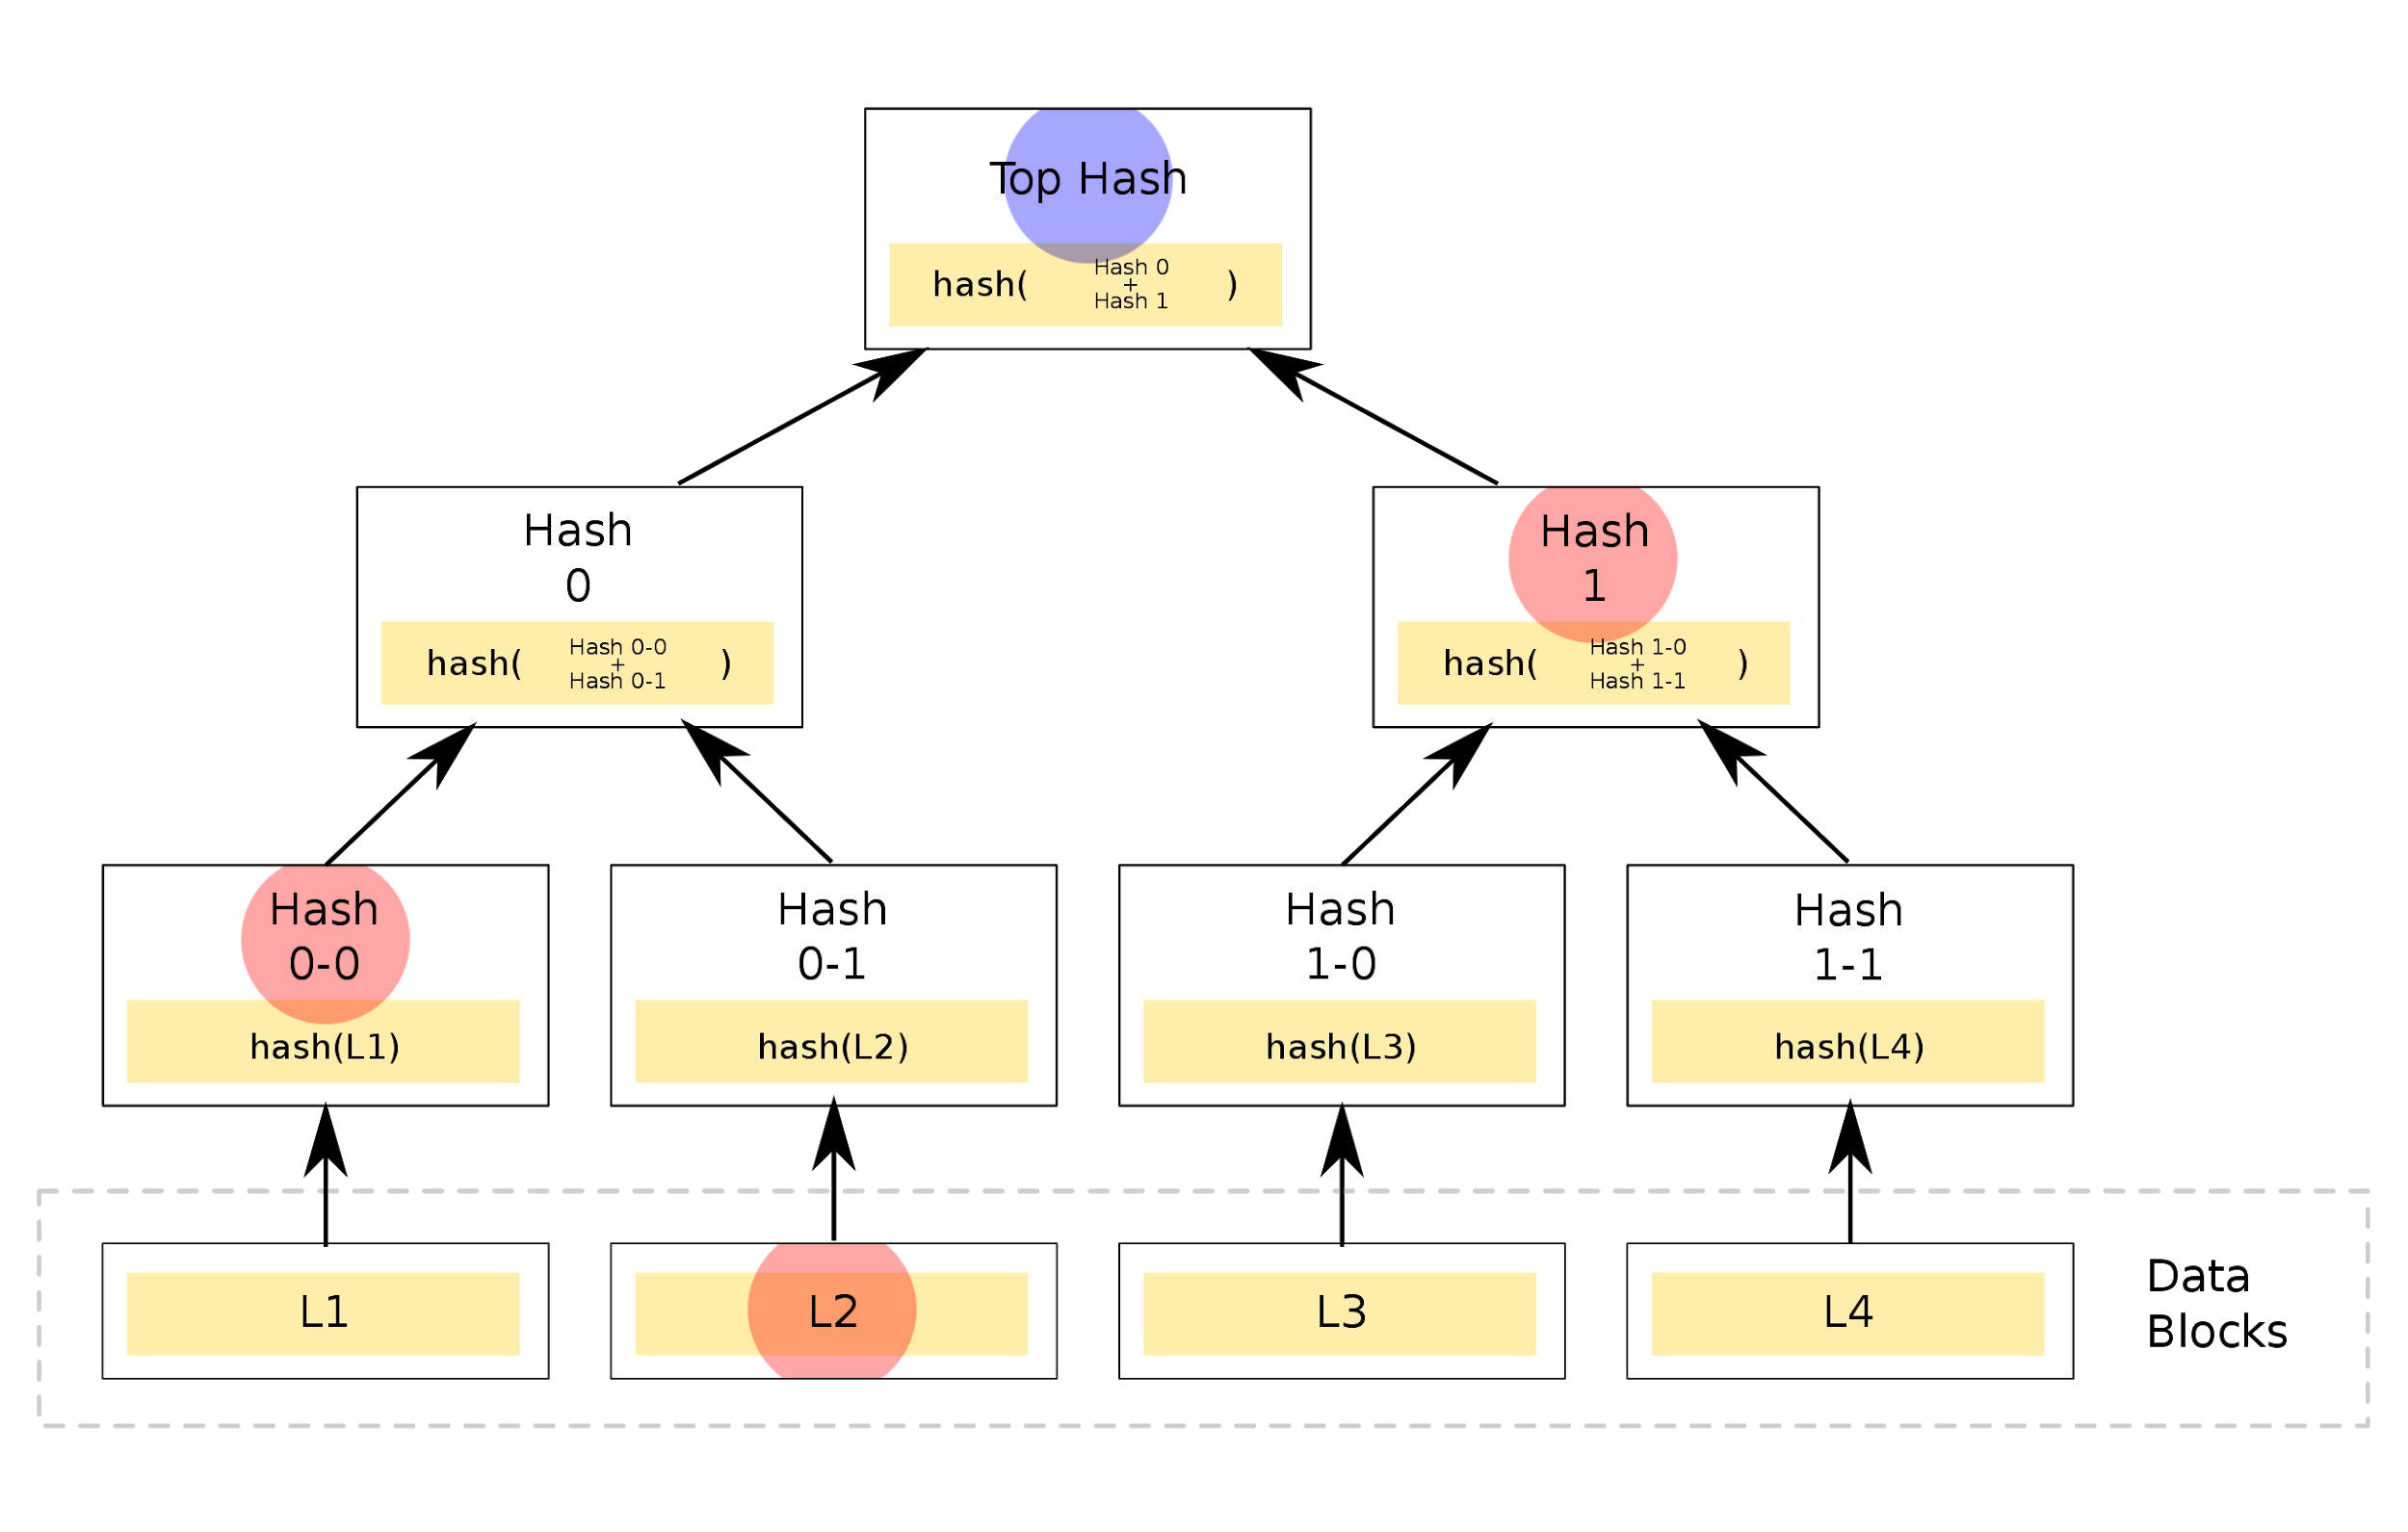
\includegraphics[width=\textwidth]{img/hash-merkle-tree}
    \caption[Merkleho strom pro~hashe]{Merkleho strom pro~veřejné klíče. Je zveřejněn pouze vršek stromu. S~podpisem L2 se zveřejní pouze ty hashe které jsou nutné k~ověření vrcholu (0-0, 1).}
\end{figure}

% TODO Možná ještě Winternitz OTS?


\clearpage
\section{V~souvislosti s~nařízením eIDAS vysvětlete pojmy -- elektronický podpis, zaručený elektronický podpis a kvalifikovaný elektronický podpis, elektronická pečeť, elektronické časové razítko.}

\subsection{Elektronický podpis}

Za~elektronický podpis může být označeno cokoliv, co má elektronickou podobu a co je použito jako podpis dané osoby.
Nezaručuje jednoznačné spojení s~podepisující osobou.

Jde např. o~napsání jména na~konec e-mailu nebo vystupování pod~svou identitou na~Facebooku.


\subsection{Zaručený elektronický podpis}

Zaručený elektronický podpis musí být jednoznačně spojen s~podepisující osobu a musí umožňit její identifikací.
Musí být vytvořen pomocí vydaného certifikátu (vydaného jakkoliv: ať kvalifikovaným poskytovatelem, tak svépomocí).


\subsection{Kvalifikovaný elektronický podpis}

Kvalifikovaný elektronický podpis je vytvořený kvalifikovaným prostředkem pro~vytváření elektronických podpisů a je založen na~kvalifikovaném certifikátu pro~elektronické podpisy.
Kvalifikovaný certifikát je vydaný kvalifikovaným poskytovatelem služeb vytvářejících důvěru (tj. mu byl státním orgánem udělen takový status; v~ČR jsou v~současnosti čtyři).

V~ČR mohou kvalifikované elektronické podpisy vydávat:
\vspace*{-0.5em}\begin{itemize}
\item První certifikační autorita, a. s.
\item Česká pošta, s. p. (služba Postsignum)
\item eIdentity a. s.
\item Národní certifikační autorita (poskytovatel: Správa základních registrů)
\end{itemize}


\subsection{Elektronická pečeť}

Elektronická pečeť se vydává pouze právnickým osobám.
PO může svou pečetí opatřit pouze to, čeho je původcem.
Princip zůstává totožný s~podepisováním elektronickým podpisem.


\subsection{Elektronické časové razítko}

Časové razítko je ekvivalent časového určení a místa vlastního podpisu na~listině (což elektronický podpis neřeší).
Zajišťuje důkaz o~existenci dokumentu a~validitu podepisujícího certifikátu v~daném čase (pomocí hashe dokumentu).

Razítko je nutné pro~poskytování elektronických notářských služeb a zajištění dlouhodobé archivace elektronicky podepsaných dokumentů.
Je vydáváno autoritou pro~vydávání časových razítek (TSA, \emph{Time Stamping Authority}).
Je nutné dokumenty pravidelně přerazítkovat, pokud má být zachována jejich platnost.

Obsahem razítka je jméno vydavatele (autority), sériové číslo razítka, kontrolní součet dokumentu a čas.

\subsubsection{Zdroj času}

Zdroj času musí pocházet z~oficiálního a důvěryhodného zdroje, např. od~národní časové autority, nesmí být možné ho při~přenosu změnit a zdroj času musí být možné zpětně dohledat celou hierarchií.


\clearpage
\section{Autentizační protokoly -- na~jakém principu pracují, využívané proměnné parametry, hodnocení jejich bezpečnosti (BAN logika).}

\subsection{Princip}

Autentizační protokoly fungují na~principu výzva--odpověď mezi dvěma entitami (klient, server), případně s~využitím třetí důvěryhodné strany.
Ověřují správnost a čerstvost autentizačního požadavku: pro~záruku čerstvosti se využívají náhodná nebo sekvenční čísla nebo časová razítka.


\subsection{Využívané proměnné parametry}

\uline{Sekvenční číslo} je tajné; při~každém dalším požadavku se inkrementuje.
V~případě desynchronizace je nutné využít nějaký autentizační protokol k~synchronizaci zpět.

\uline{Časové razítko} pracuje s~maximálním povoleným zpožděním (\emph{acceptance window}) přijaté zprávy.
Přijatá razítka jsou lokálně ukládána pro~případ útoku přehráním (během povoleného časového okna nebo při~změně času u~ověřovatele).

\uline{Nonce} synchronizaci nezajišťuje; ověřovatel ho zašle protistraně a~ta ho vrátí zpět v~odpovědi, poté je vyřazeno aby nemohlo být použito znovu.
Pokud je dost velký (128~bit), náhodný výběr snižuje pravděpodobnost výběru na~zanedbatelnou úroveň.


\subsection{Hodnocení bezpečnosti -- BAN logika}

BAN logika slouží k~formálnímu zápisu bezpečnosti autentizačních protokolů, je určena pro~symetrickou i asymetrickou kryptografii.
Zabývá se protokoly na~abstraktní úrovni: neřeší implementaci protokolu a~problémy s~tím spjaté.

\subsubsection{Otázky BAN logiky}

\begin{enumerate}
    \item Čeho chce zkoumaný protokol dosáhnout?
    \item Potřebuje zkoumaný protokol více předpokladů než jiný protokol?
    \item Vykonává zkoumaný protokol cokoliv nepotřebného, jenž by mohlo být vypuštěno bez~ohrožení bezpečnosti?
    \item Šifruje zkoumaný protokol něco, co by mohlo být zasláno v~otevřené formě bez~ohrožení bezpečnosti?
\end{enumerate}

\subsubsection{Konstrukce BAN logiky}

\begin{tabularx}{\textwidth}{lX}
$P$ věří $X$ & $P$ věří výroku $X$, může jednat jako by $X$ bylo pravdivé. \\
$P$ vidí $X$ & $P$ přijal zprávu obsahující výrok $X$, jenž může přečíst a~zopakovat. \\
$P$ vyslovil $X$ & $P$ někdy zaslal zprávu obsahující výrok $X$. \\
$P$ jurisdikce $X$ & $P$ je autorita k~$X$ a~měl by být důvěryhodný. \\
& \emph{Např. servery generující klíče pro~další entity.} \\
nový $X$ & $X$ nebylo nikdy odesláno. \\
$P \stackrel{K}{\leftrightarrow} Q$ & $P$ a~$Q$ mohou použít sdílený klíč $K$ ke~komunikaci. \\
$\stackrel{K}{\rightarrow} P$ & $P$ má veřejný klíč $K$. \\
$P \stackrel{X}{\rightleftharpoons} Q$ & $X$ je tajemství známé pouze $P$ a~$Q$. \\
$\{X\}_K$ & $X$ je zašifrován klíčem $K$ \\
$\left<X\right>_Y$ & $X$ je kombinovaný s~výrokem $Y$. $Y$ je tajné a~jeho přítomnost ověřuje identitu toho kdo vyslovil $Y$. Je to důkaz původu výroku $X$. \\
\end{tabularx}

\begin{tabular}{ll}
význam zprávy (sdílené klíče)
& $P$ věří $Q \stackrel{K}{\leftrightarrow} P$, $P$ vidí $\{X\}_K$ \\
& $P$ věří $Q$ vyslovilo $X$ \\
význam zprávy (veřejné klíče) & $P$ věří $\stackrel{K}{\rightarrow} Q$, $P$ vidí $\{X\}_{K^{-1}}$ \\
& $P$ věří $Q$ vyslovilo $X$ \\
význam zprávy (sdílená tajemství) & $P$ věří $Q \stackrel{Y}{\rightleftharpoons} P$, $P$ vidí $\left<X\right>_Y$ \\
& $P$ věří $Q$ vyslovilo $X$ \\

ověření aktuálnosti zprávy
& $P$ věří nový $X$, $P$ věří $Q$ vyslovilo $X$ \\
& $P$ věří $Q$ věří $X$ \\

jurisdikce
& $P$ věří $Q$ jurisdikce $X$, $P$ věří $Q$ věří $X$ \\
& $P$ věří $X$ \\

důvěra k~množině výroků
& $P$ věří množině výroku pokud věří každému zvlášť \\

novost celého výroku
& Pokud je část výroku nová, celý výrok je nový \\
\end{tabular}

\subsubsection{Analýza protokolů pomocí BAN logiky}

\begin{enumerate}
\item Z~původního protokolu se odvodí idealizovaná verze protokolu.
\item Sepíší se předpoklady ohledně počátečního stavu.
\item Logické formule se připojí k~jednotlivým výrokům jako tvrzení o~stavu systému po~každém kroku.
\item Logické výchozí předpoklady (postuláty) se aplikují na~předpoklady a~tvrzení za~účelem zjištění toho, v~co věří jednotlivé strany.
\end{enumerate}
